% !TEX root = ../10.DOUBLE-PIPE.tex
\section{EXPERIMENTAL PRINCIPLE}\label{experimental-principle}

Heat exchanging in a double-pipe heat exchanger is an example of complex heat transfer, where heat is exchanged between two fluid flows through a metal wall. This process involves:
\begin{itemize}
    \item Convectional heat transfer from the hot stream to the wall.
    \item Conduction through the metal wall.
    \item Convectional heat transfer from the wall to the cold stream.
\end{itemize}

\subsection{Heat Balance Equation}\label{heat-balance-equation}

The heat balance equation for the two fluid streams is given by:
\begin{equation}
    Q = G_1 C_{p1}(t_{1\text{in}} - t_{1\text{out}}) = G_2 C_{p2}(t_{2\text{out}} - t_{2\text{in}}) \quad [W]
\end{equation}
Where:
\begin{itemize}
    \item $G_1, G_2$: Hot and cold stream mass flow rate $[kg/s]$.
    \item $C_{p1}, C_{p2}$: Average specific heat capacity of hot and cold stream $[J/kg \cdot K]$.
    \item $t_{1\text{in}}, t_{1\text{out}}$: Inlet and outlet temperature of the hot stream $[^\circ C]$.
    \item $t_{2\text{in}}, t_{2\text{out}}$: Inlet and outlet temperature of the cold stream $[^\circ C]$.
\end{itemize}

\subsection{Heat Transfer Equation}\label{heat-transfer-equation}

The heat transfer is also determined by:
\begin{equation}
    Q = K_l \cdot \Delta t_{\text{log}} \cdot L
\end{equation}
Where:
\begin{itemize}
    \item $L$: Effective tube length $[m]$.
    \item $K_l$: Experimental linear heat transfer coefficient $[W/m \cdot K]$.
    \item $\Delta t_{\text{log}}$: Logarithmic Mean Temperature Difference (LMTD) $[K]$.
\end{itemize}

\subsection{Logarithmic Mean Temperature Difference (LMTD)}\label{lmtd}

The LMTD is defined as:
\begin{equation}
    \Delta t_{\text{log}} = \frac{\Delta t_{\text{max}} - \Delta t_{\text{min}}}{\ln\left(\frac{\Delta t_{\text{max}}}{\Delta t_{\text{min}}}\right)}
\end{equation}
For counter-flow:
\begin{equation}
    \Delta t_{\text{max}} = t_{1\text{in}} - t_{2\text{out}}; \quad \Delta t_{\text{min}} = t_{1\text{out}} - t_{2\text{in}}
\end{equation}

\subsection{Overall Heat Transfer Coefficient, $K_l^*$}\label{overall-heat-transfer-coefficient}

The theoretical overall linear heat transfer coefficient $K_l^*$ is calculated from the individual thermal transmittance coefficients of each stream and the wall conduction:
\begin{equation}
    K_l^* = \frac{\pi}{\frac{1}{\alpha_1 d_1} + \frac{1}{2\lambda_w} \ln\left(\frac{d_2}{d_1}\right) + \frac{1}{\alpha_2 d_{2}}}
\end{equation}
Where:
\begin{itemize}
    \item $\alpha_1, \alpha_2$: Convective heat transfer coefficients $[W/m^2 \cdot K]$.
    \item $\lambda_w$: Thermal conductivity of the wall (copper) $[W/m \cdot K]$.
    \item $d_1, d_2$: Internal and external diameter of the inner tube $[m]$.
\end{itemize}

\subsection{Thermal Transmittance Coefficient ($\alpha$)}\label{thermal-transmittance}

The coefficient $\alpha$ is determined from the Nusselt number ($Nu$):
\begin{equation}
    \alpha = \frac{Nu \cdot \lambda}{l}
\end{equation}
Where:
\begin{itemize}
    \item $\lambda$: Thermal conductivity of the fluid $[W/m \cdot K]$.
    \item $l$: Characteristic dimension (e.g., equivalent diameter) $[m]$.
\end{itemize}

The Reynolds number ($Re$) determines the flow mode:
\begin{equation}
    Re = \frac{w \cdot l}{\nu}
\end{equation}
Where $w$ is the flow velocity $[m/s]$ and $\nu$ is the kinematic viscosity $[m^2/s]$.

The equivalent diameter $d_{\text{eq}}$ for non-circular sections (like the annulus in Tube C) is:
\begin{equation}
    d_{\text{eq}} = \frac{4F}{\Pi}
\end{equation}
Where $F$ is the cross-sectional area and $\Pi$ is the wetted circumference.

\subsection{Dimensionless Numbers Correlation}\label{correlations}

The heat transfer coefficients are determined using dimensionless correlations specific to the flow geometry and regime.

\subsubsection{Nusselt Number ($Nu$)}\label{nu-number}

The Nusselt number represents the ratio of convective to conductive heat transfer.

\textbf{Cross Flow (Tube B):}
\begin{itemize}
    \item $5 < Re < 10^3$: $Nu = 0.5 \cdot Re^{0.5} \cdot Pr^{0.38} \cdot \left(\frac{Pr}{Pr_w}\right)^{0.25} \cdot \epsilon_\psi$
    \item $10^3 < Re < 2 \cdot 10^5$: $Nu = 0.25 \cdot Re^{0.6} \cdot Pr^{0.38} \cdot \left(\frac{Pr}{Pr_w}\right)^{0.25} \cdot \epsilon_\psi$
    \item $2 \cdot 10^5 < Re < 2 \cdot 10^6$: $Nu = 0.023 \cdot Re^{0.8} \cdot Pr^{0.37} \cdot \left(\frac{Pr}{Pr_w}\right)^{0.25} \cdot \epsilon_\psi$
\end{itemize}

\textbf{Longitudinal Flow (Tube C):}
\begin{itemize}
    \item \textbf{Laminar Flow ($Re < 2320$):}
    \begin{equation}
        Nu = 0.15 \cdot Re^{0.33} \cdot Pr^{0.43} \cdot Gr^{0.1} \cdot \left(\frac{Pr}{Pr_w}\right)^{0.25} \cdot \epsilon_l
    \end{equation}
    \item \textbf{Transition Flow ($2320 < Re < 10000$):}
    \begin{equation}
        Nu = K \cdot Pr^{0.43} \cdot \left(\frac{Pr}{Pr_w}\right)^{0.25}
    \end{equation}
    Where $K$ depends on $Re$ as shown in Table \ref{tab:re-k-correlation}.

    \begin{table}[H]
        \centering
        \caption{Determining $K$ according to $Re$ number}
        \label{tab:re-k-correlation}
        \begin{tabular}{|c|c|c|c|c|c|c|c|c|c|}
            \hline
            \textbf{Re} & 2200 & 2500 & 3000 & 4000 & 5000 & 6000 & 7000 & 8000 & 10000 \\ \hline
            \textbf{K}  & 2.2  & 4.5  & 10.5 & 18   & 23.5 & 28   & 31   & 32   & 33    \\ \hline
        \end{tabular}
    \end{table}

    \item \textbf{Turbulent Flow ($Re > 10^4$):}
    \begin{equation}
        Nu = 0.021 \cdot Re^{0.8} \cdot Pr^{0.43} \cdot \left(\frac{Pr}{Pr_w}\right)^{0.25} \cdot \epsilon_l
    \end{equation}
    Where the coefficient $\epsilon_l$ depends on the ratio $l/d$ as shown in Table \ref{tab:ld-epsilon}.

    \begin{table}[H]
        \centering
        \caption{Coefficient $\epsilon_l$ dependence on the ratio $l/d$}
        \label{tab:ld-epsilon}
        \begin{tabular}{|c|c|c|c|c|c|c|c|c|c|}
            \hline
            \textbf{$l/d$}       & 1   & 2   & 5    & 10   & 15   & 20   & 30   & 40   & 50  \\ \hline
            \textbf{$\epsilon_l$} & 1.9 & 1.7 & 1.44 & 1.28 & 1.18 & 1.13 & 1.05 & 1.02 & 1.0 \\ \hline
        \end{tabular}
    \end{table}
\end{itemize}

\subsubsection{Prandtl Number ($Pr$)}\label{pr-number}

The Prandtl number relates the momentum diffusivity to thermal diffusivity:
\begin{equation}
    Pr = \frac{\nu}{a} = \frac{\mu \cdot C_p}{\lambda}
\end{equation}
Where $\nu$ is kinematic viscosity and $a$ is thermal diffusivity.

\subsubsection{Grashof Number ($Gr$)}\label{gr-number}

The Grashof number approximates the ratio of the buoyancy to viscous force acting on a fluid:
\begin{equation}
    Gr = \frac{g \cdot \beta \cdot \Delta t \cdot l^3}{\nu^2}
\end{equation}
Where:
\begin{itemize}
    \item $g$: Gravitational acceleration ($9.81 m/s^2$).
    \item $\beta$: Volume expansion coefficient ($1/K$).
    \item $\Delta t$: Temperature difference between wall and fluid.
\end{itemize}

\subsection{Temperature Distribution Diagram}\label{temp-dist}

The figure below illustrates the temperature gradient across the heat transfer surfaces.

\begin{figure}[H]
    \centering
    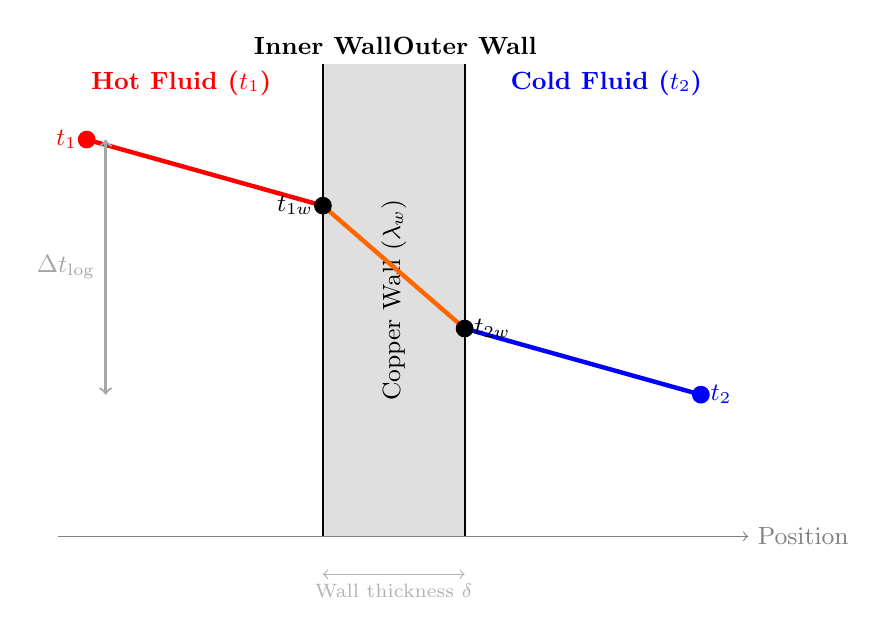
\begin{tikzpicture}[scale=1.2]
        % --- Copper wall region (wider, clearly visible) ---
        \fill[gray!25] (2.5,0) rectangle (4.0,5);

        % --- Wall boundary lines ---
        \draw[thick, black] (2.5,0) -- (2.5,5);
        \draw[thick, black] (4.0,0) -- (4.0,5);

        % --- Wall labels (above) ---
        \node[above, font=\small\bfseries] at (2.5,5) {Inner Wall};
        \node[above, font=\small\bfseries] at (4.0,5) {Outer Wall};

        % --- Copper Wall label (inside grey zone) ---
        \node[font=\small, rotate=90] at (3.25,2.5) {Copper Wall ($\lambda_w$)};

        % --- Fluid zone labels ---
        \node[font=\small\bfseries, red]  at (1.0,4.8) {Hot Fluid ($t_1$)};
        \node[font=\small\bfseries, blue] at (5.5,4.8) {Cold Fluid ($t_2$)};

        % --- Temperature profile: hot side ---
        \draw[ultra thick, red]   (0.0,4.2) -- (2.5,3.5);  % Hot fluid bulk to inner wall

        % --- Temperature drop through copper wall ---
        \draw[ultra thick, orange!80!red] (2.5,3.5) -- (4.0,2.2);  % Conduction through wall

        % --- Temperature profile: cold side ---
        \draw[ultra thick, blue]  (4.0,2.2) -- (6.5,1.5);  % Outer wall to cold fluid bulk

        % --- Key temperature points ---
        \filldraw[red]    (0.0,4.2) circle (2.5pt) node[left,  font=\small] {$t_1$};
        \filldraw[black]  (2.5,3.5) circle (2.5pt) node[left,  font=\small] {$t_{1w}$};
        \filldraw[black]  (4.0,2.2) circle (2.5pt) node[right, font=\small] {$t_{2w}$};
        \filldraw[blue]   (6.5,1.5) circle (2.5pt) node[right, font=\small] {$t_2$};

        % --- LMTD annotation (double-headed arrow) ---
        \draw[<->, thick, gray!70] (0.2,4.2) -- (0.2,1.5) node[midway, left, font=\small] {$\Delta t_{\log}$};

        % --- x-axis baseline ---
        \draw[->, thin, gray] (-0.3,0) -- (7.0,0) node[right, font=\small] {Position};

        % --- Dimension braces for wall thickness ---
        \draw[<->, thin, gray!60] (2.5,-0.4) -- (4.0,-0.4) node[midway, below, font=\scriptsize] {Wall thickness $\delta$};
    \end{tikzpicture}
    \caption{Temperature distribution across the double-pipe heat exchanger wall}
    \label{fig:temp-dist}
\end{figure}

\subsection{Iterative Wall Temperature Calculation}\label{wall-temp-calc}

If the wall temperatures $t_{1w}, t_{2w}$ are not directly measured, they are determined iteratively using:
\begin{equation}
    \Delta t_1 = t_1 - t_{1w} = \frac{Q}{\alpha_1 \cdot F_1}
\end{equation}
\begin{equation}
    \Delta t_2 = t_{2w} - t_2 = \frac{Q}{\alpha_2 \cdot F_2}
\end{equation}
The procedure is repeated until the error between assumed and calculated $\Delta t$ is less than 5\%.
